\documentclass{article}\usepackage[]{graphicx}\usepackage[]{color}
%% maxwidth is the original width if it is less than linewidth
%% otherwise use linewidth (to make sure the graphics do not exceed the margin)
\makeatletter
\def\maxwidth{ %
  \ifdim\Gin@nat@width>\linewidth
    \linewidth
  \else
    \Gin@nat@width
  \fi
}
\makeatother

\definecolor{fgcolor}{rgb}{0.345, 0.345, 0.345}
\newcommand{\hlnum}[1]{\textcolor[rgb]{0.686,0.059,0.569}{#1}}%
\newcommand{\hlstr}[1]{\textcolor[rgb]{0.192,0.494,0.8}{#1}}%
\newcommand{\hlcom}[1]{\textcolor[rgb]{0.678,0.584,0.686}{\textit{#1}}}%
\newcommand{\hlopt}[1]{\textcolor[rgb]{0,0,0}{#1}}%
\newcommand{\hlstd}[1]{\textcolor[rgb]{0.345,0.345,0.345}{#1}}%
\newcommand{\hlkwa}[1]{\textcolor[rgb]{0.161,0.373,0.58}{\textbf{#1}}}%
\newcommand{\hlkwb}[1]{\textcolor[rgb]{0.69,0.353,0.396}{#1}}%
\newcommand{\hlkwc}[1]{\textcolor[rgb]{0.333,0.667,0.333}{#1}}%
\newcommand{\hlkwd}[1]{\textcolor[rgb]{0.737,0.353,0.396}{\textbf{#1}}}%

\usepackage{framed}
\makeatletter
\newenvironment{kframe}{%
 \def\at@end@of@kframe{}%
 \ifinner\ifhmode%
  \def\at@end@of@kframe{\end{minipage}}%
  \begin{minipage}{\columnwidth}%
 \fi\fi%
 \def\FrameCommand##1{\hskip\@totalleftmargin \hskip-\fboxsep
 \colorbox{shadecolor}{##1}\hskip-\fboxsep
     % There is no \\@totalrightmargin, so:
     \hskip-\linewidth \hskip-\@totalleftmargin \hskip\columnwidth}%
 \MakeFramed {\advance\hsize-\width
   \@totalleftmargin\z@ \linewidth\hsize
   \@setminipage}}%
 {\par\unskip\endMakeFramed%
 \at@end@of@kframe}
\makeatother

\definecolor{shadecolor}{rgb}{.97, .97, .97}
\definecolor{messagecolor}{rgb}{0, 0, 0}
\definecolor{warningcolor}{rgb}{1, 0, 1}
\definecolor{errorcolor}{rgb}{1, 0, 0}
\newenvironment{knitrout}{}{} % an empty environment to be redefined in TeX

\usepackage{alltt}

\usepackage{fancyhdr} % Required for custom headers
\usepackage{lastpage} % Required to determine the last page for the footer
\usepackage{extramarks} % Required for headers and footers
\usepackage{graphicx} % Required to insert images
\usepackage{hyperref}
\usepackage{amsmath} %for binomial pdf
\usepackage{parskip} % so that there's space bw paragraphs
\usepackage{float}
\usepackage{amsfonts}

% Margins
\topmargin=-0.45in
\evensidemargin=0in
\oddsidemargin=0in
\textwidth=6.5in
\textheight=9.0in
\headsep=0.25in 

\linespread{1.1} % Line spacing

% Set up the header and footer
\pagestyle{fancy}
\lhead{STAT 532: Bayes} % Top left header
\chead{HW 2} % Top center header
\rhead{Andrea Mack} % Top right header
\lfoot{09/26/2016} % Bottom left footer
\cfoot{} % Bottom center footer
\rfoot{Page\ \thepage\ of\ \pageref{LastPage}} % Bottom right footer
\renewcommand\headrulewidth{0.4pt} % Size of the header rule
\renewcommand\footrulewidth{0.4pt} % Size of the footer rule

\setlength\parindent{0pt} % Removes all indentation from paragraphs
\setlength\parskip{0.5cm}
\restylefloat{table}

%----------------------------------------------------------------------------------------
%	DOCUMENT STRUCTURE COMMANDS
%	Skip this unless you know what you're doing
%----------------------------------------------------------------------------------------

% Header and footer for when a page split occurs within a problem environment
\newcommand{\enterProblemHeader}[1]{
\nobreak\extramarks{#1}{#1 continued on next page\ldots}\nobreak
\nobreak\extramarks{#1 (continued)}{#1 continued on next page\ldots}\nobreak
}

% Header and footer for when a page split occurs between problem environments
\newcommand{\exitProblemHeader}[1]{
\nobreak\extramarks{#1 (continued)}{#1 continued on next page\ldots}\nobreak
\nobreak\extramarks{#1}{}\nobreak
}


%----------------------------------------------------------------------------------------%
\IfFileExists{upquote.sty}{\usepackage{upquote}}{}
\begin{document}


\begin{enumerate}
\item%1
We see that for values for p not close to 0 or 1, that the confidence level is maintained well for both sample sizes 50 and 100 in 10,000 replications. For very small and very large proportions, it is more likely to get all failures or all successes (respectively), making for no estimate of the variation in the proportion of successes. Then, the proportion, p, is contained within fewer 10,000 confidence intervals, making the confidence level not maintained as well. For the larger sample size, 100, the confidence level is more maintained on the boundaries of p than for the smaller sample size (50). I am not surprised because for the Wald Interval estimate for p to be valid (meaning maintained specified confidence level), the expected number of successes, np, needs to be large enough to have at least 10 successes and 10 failures, which does not hold on the boundaries with the sample sizes 50 and 100. For example, 0.1*100 = 1.

%maintainence of the confidence level is an asymptotic result, both in the sense of the number of simulations (10,000 here) and in the sense of the sample size. The asymptotic result in terms of sample size means that to maintain the confidence level, we need an adequately large sample size and for proportions on the boundary, an adequately large sample size is larger to ensure we get enough succeses and failures to get an estimate of the variation.


\begin{figure}[h!]
\begin{knitrout}
\definecolor{shadecolor}{rgb}{0.969, 0.969, 0.969}\color{fgcolor}

{\centering 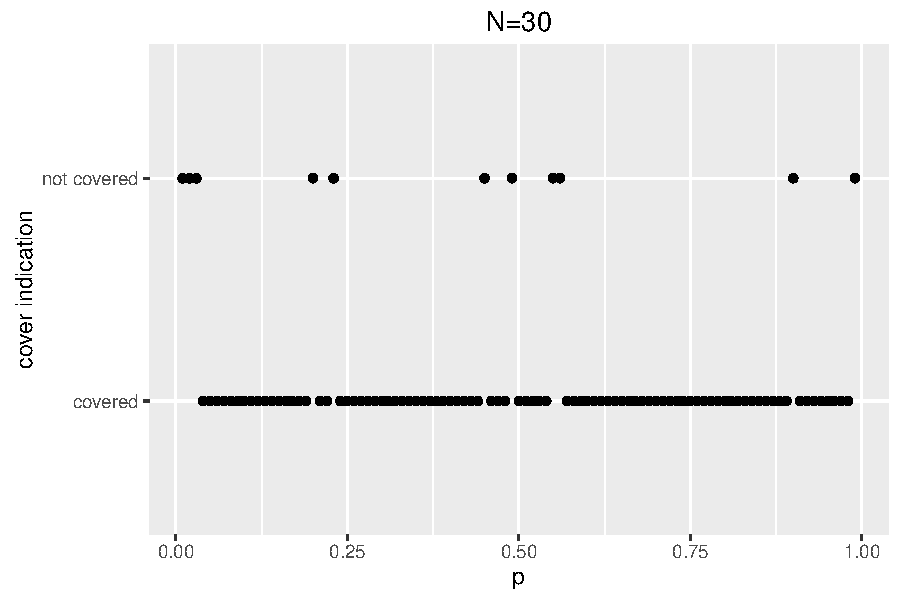
\includegraphics[width=\maxwidth]{figure/prob1_part1-1} 

}



\end{knitrout}
\end{figure}






\begin{figure}[h!]
\begin{knitrout}
\definecolor{shadecolor}{rgb}{0.969, 0.969, 0.969}\color{fgcolor}

{\centering 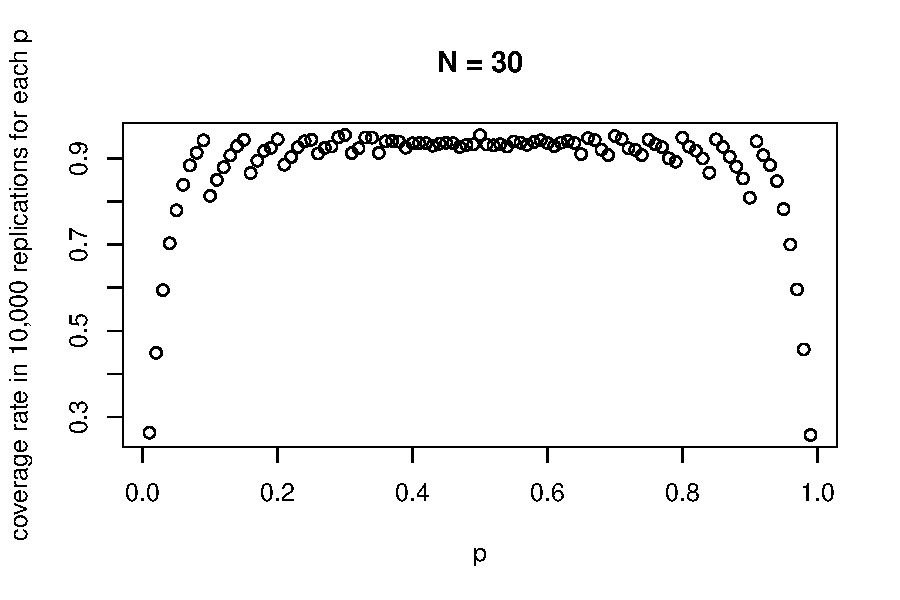
\includegraphics[width=\maxwidth]{figure/prob1_part2_plot-1} 

}



\end{knitrout}
\end{figure}






I read too quickly over the set notation, but my code did run for sample sizes between 50 and 100, so I thought I would include them as well.
\begin{knitrout}
\definecolor{shadecolor}{rgb}{0.969, 0.969, 0.969}\color{fgcolor}

{\centering 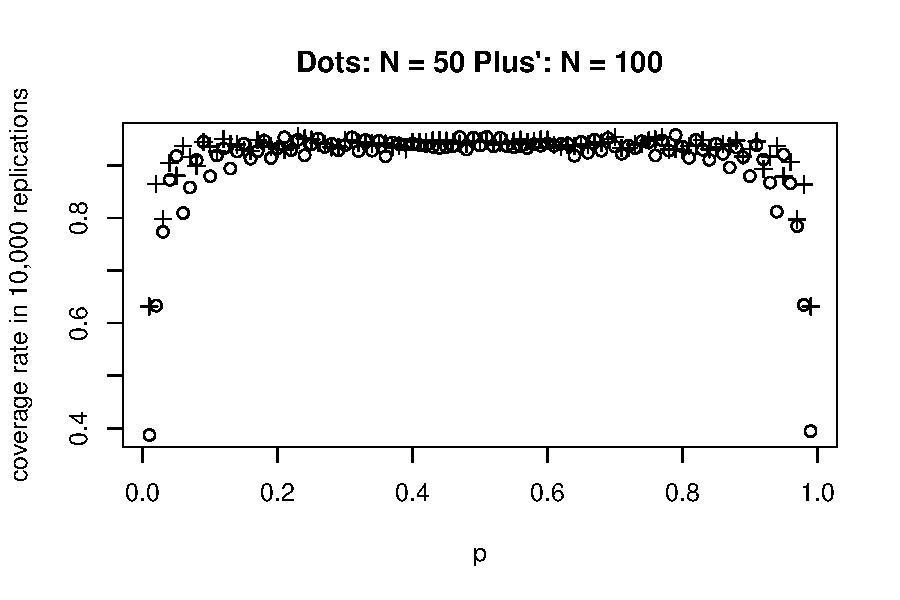
\includegraphics[width=\maxwidth]{figure/prob1_final-1} 

}




{\centering 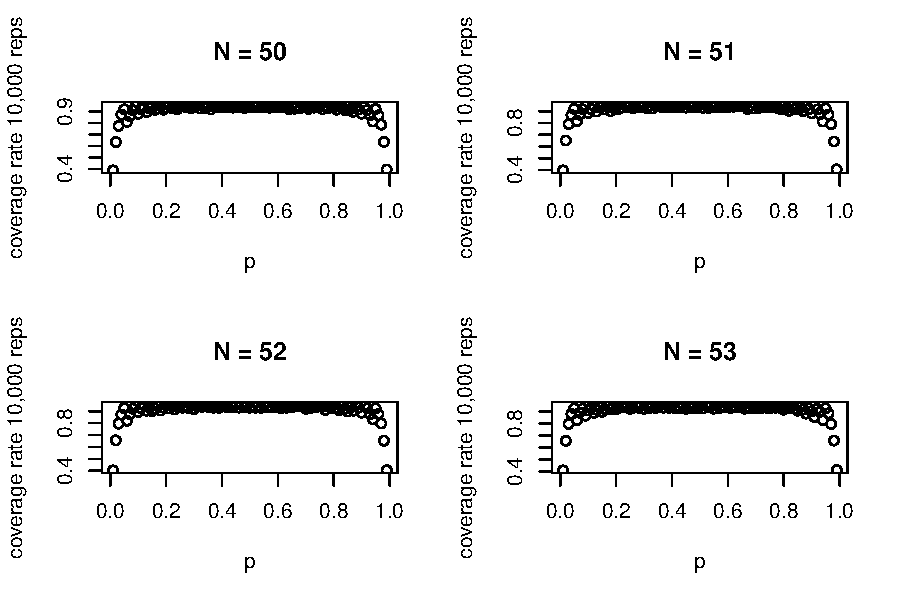
\includegraphics[width=\maxwidth]{figure/prob1_final-2} 

}




{\centering 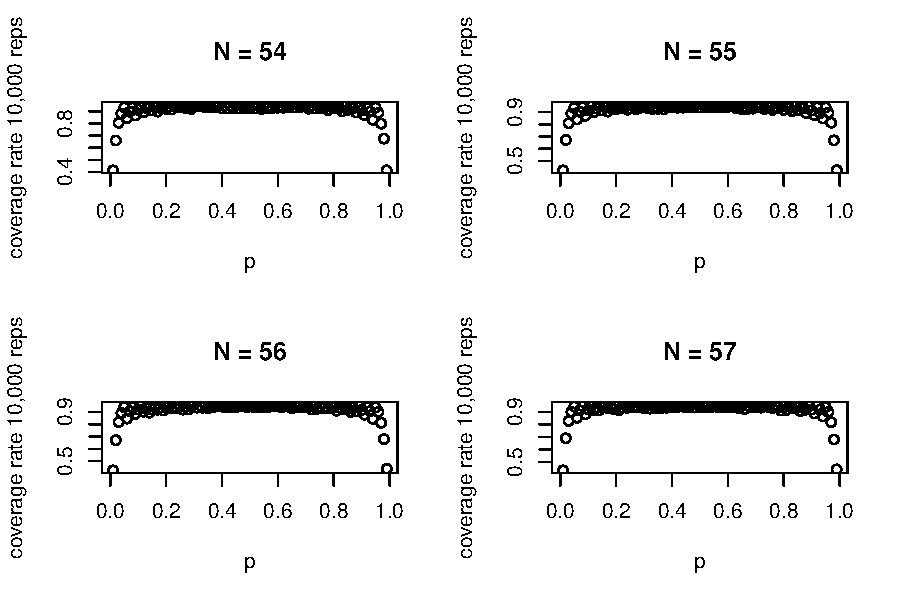
\includegraphics[width=\maxwidth]{figure/prob1_final-3} 

}




{\centering 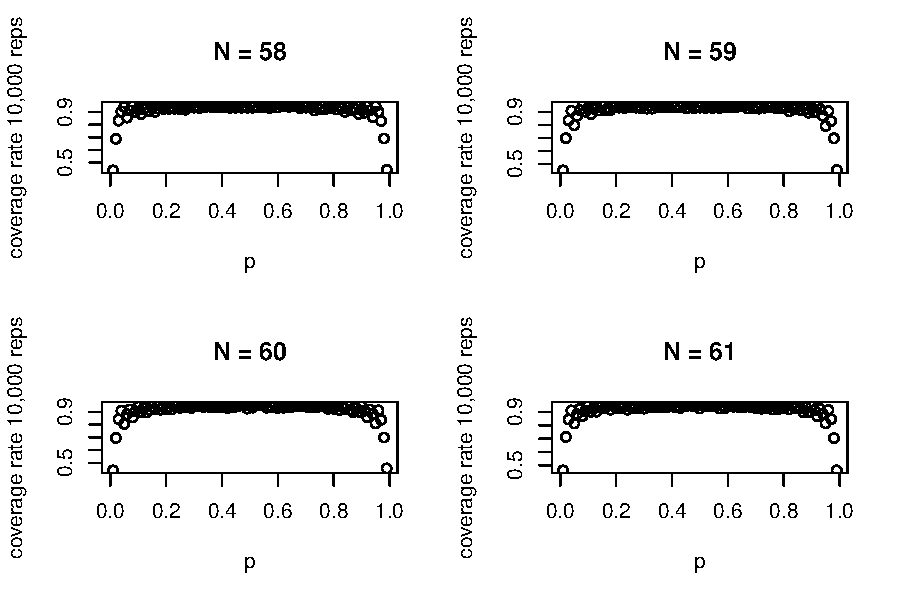
\includegraphics[width=\maxwidth]{figure/prob1_final-4} 

}




{\centering 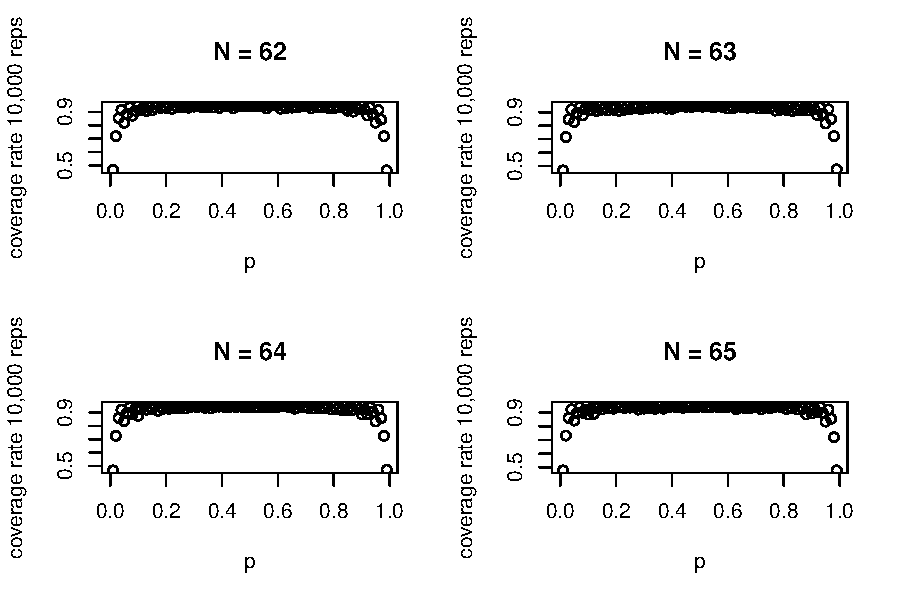
\includegraphics[width=\maxwidth]{figure/prob1_final-5} 

}




{\centering 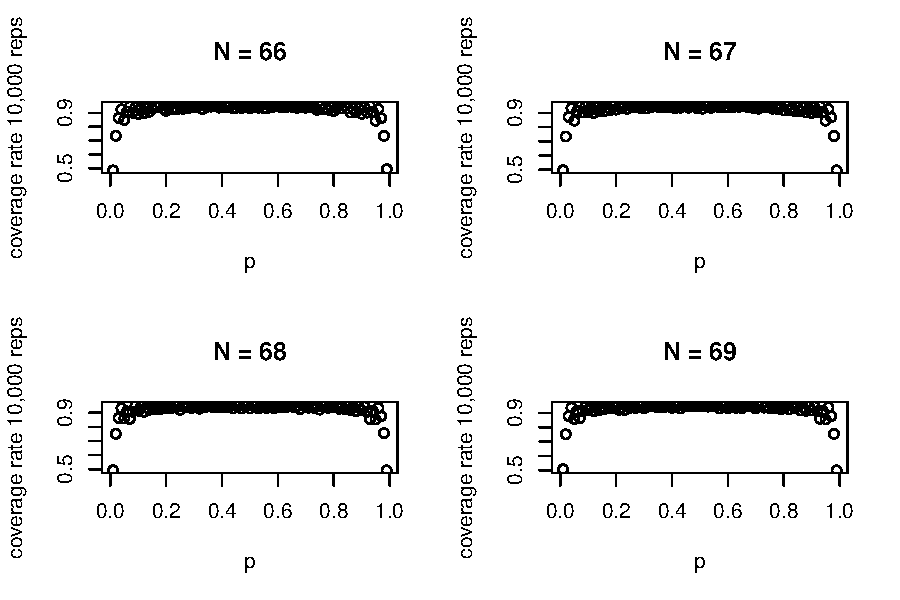
\includegraphics[width=\maxwidth]{figure/prob1_final-6} 

}




{\centering 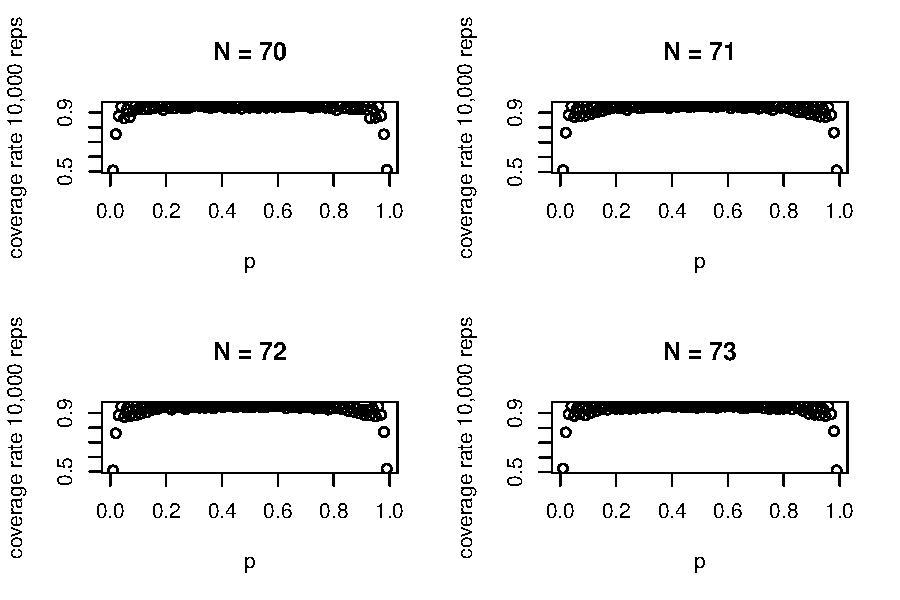
\includegraphics[width=\maxwidth]{figure/prob1_final-7} 

}




{\centering 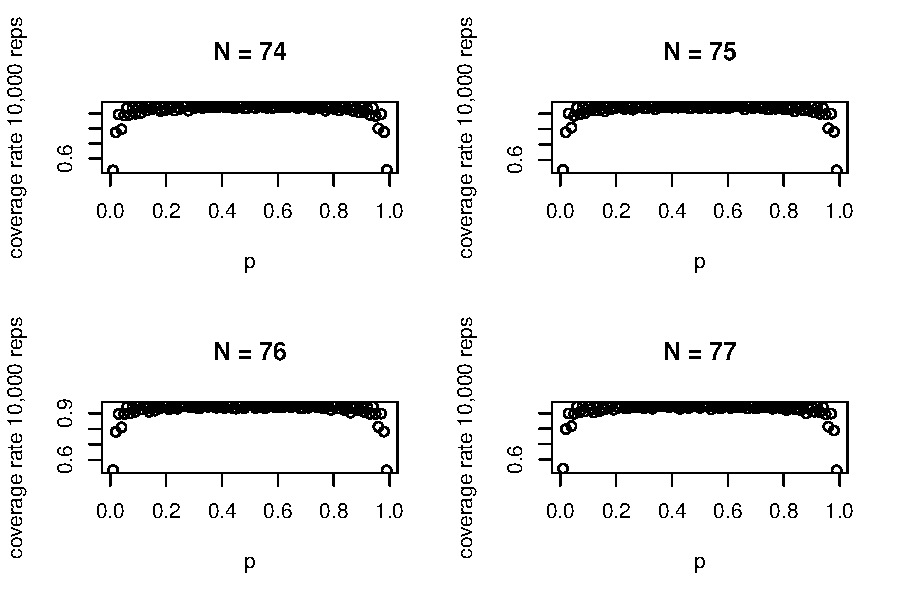
\includegraphics[width=\maxwidth]{figure/prob1_final-8} 

}




{\centering 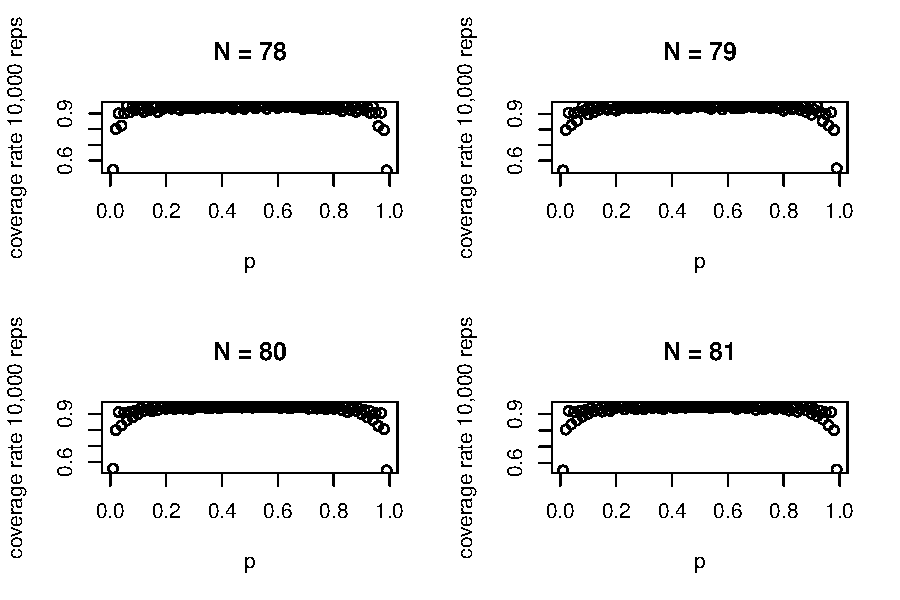
\includegraphics[width=\maxwidth]{figure/prob1_final-9} 

}




{\centering 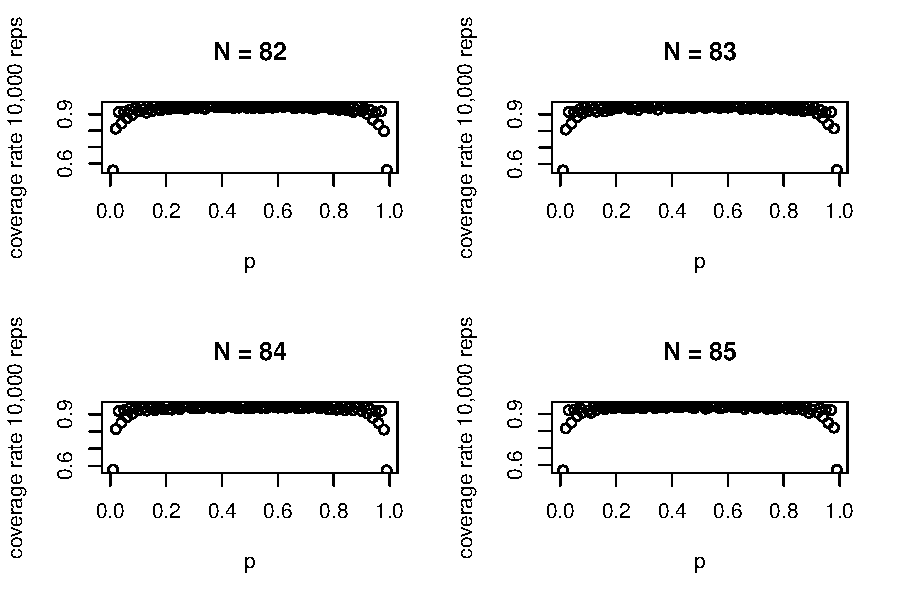
\includegraphics[width=\maxwidth]{figure/prob1_final-10} 

}




{\centering 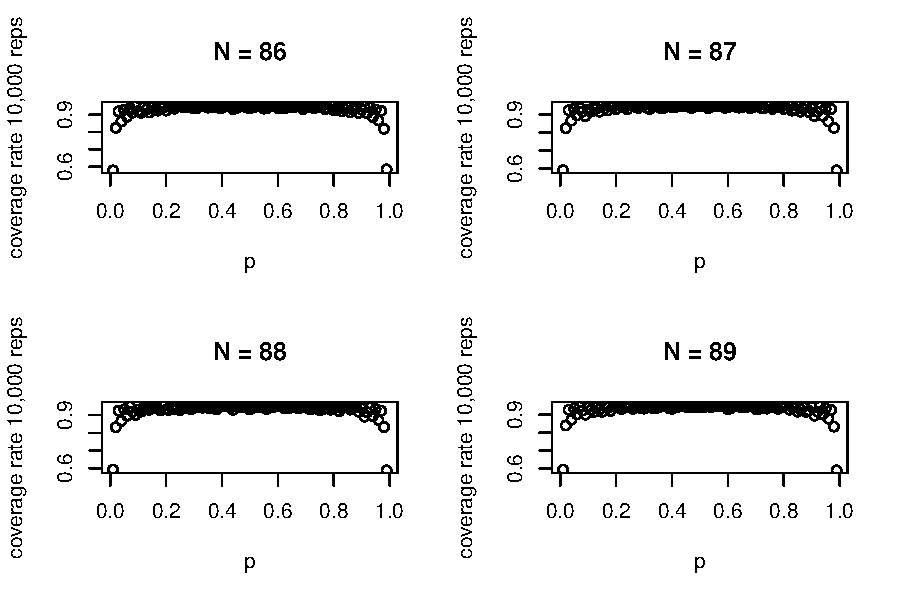
\includegraphics[width=\maxwidth]{figure/prob1_final-11} 

}




{\centering 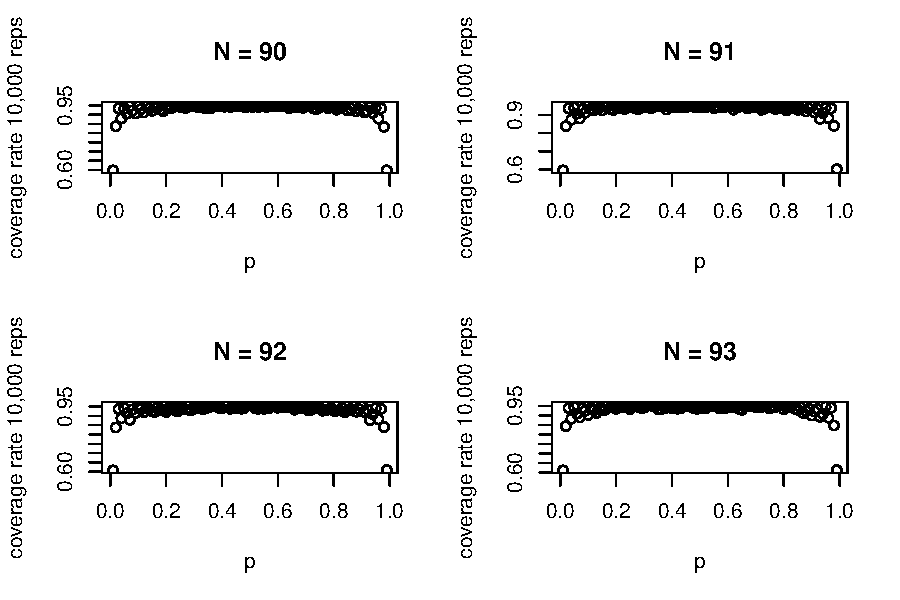
\includegraphics[width=\maxwidth]{figure/prob1_final-12} 

}




{\centering 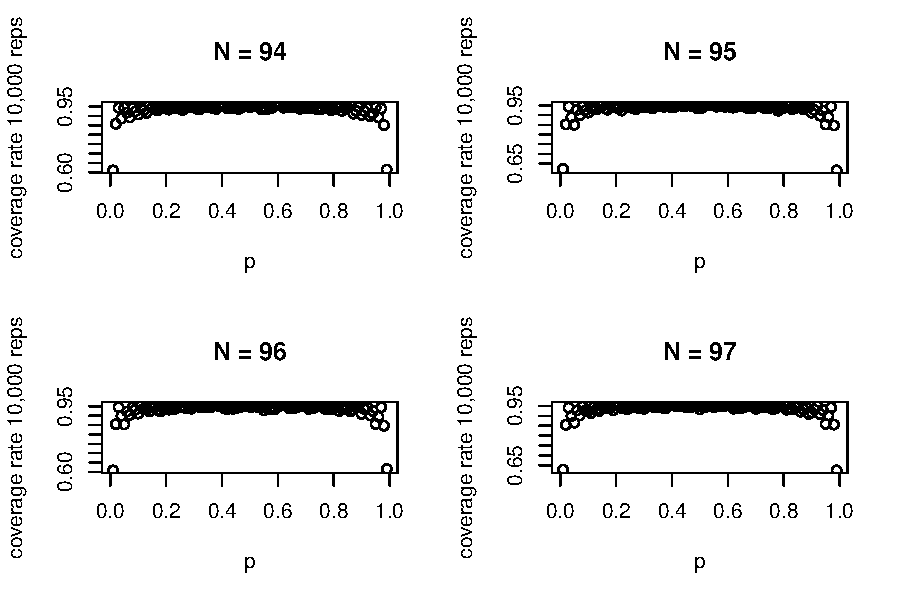
\includegraphics[width=\maxwidth]{figure/prob1_final-13} 

}




{\centering 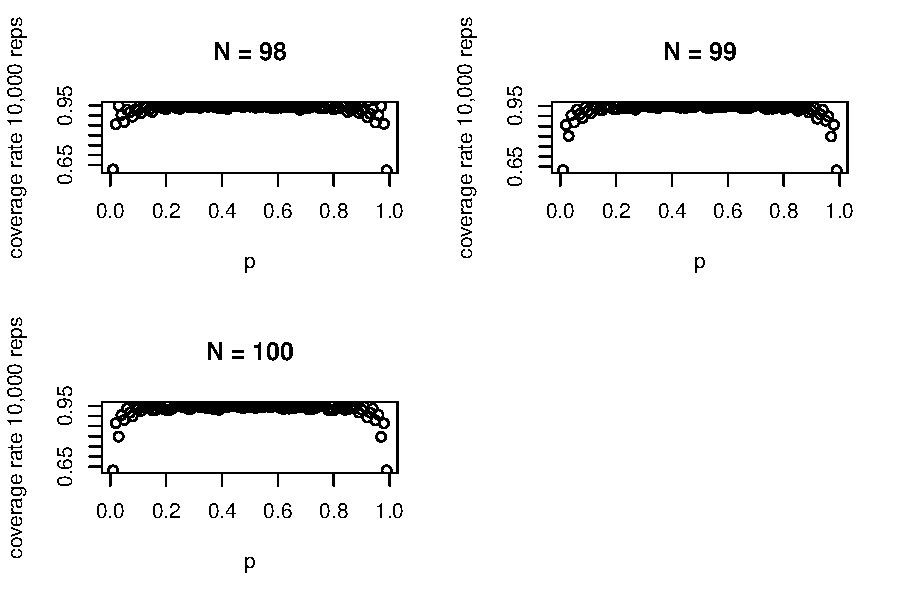
\includegraphics[width=\maxwidth]{figure/prob1_final-14} 

}



\end{knitrout}


\item%2
X $\sim$ BIN(N, $\theta$)

$\theta$ $\sim$ UNIF(0,1)

$\theta \vert$  Y $\sim$ BETA(1+$\Sigma y_{i}$, 1 + N - $\Sigma y_{i}$)

$\Lambda$ = $log(\frac{\theta}{1-\theta})$

\begin{enumerate}
\item%2a
p($\theta$) = 1 \cdot $I(\theta)_{[0,1]}$

$\theta = \frac{e^{\Lambda}}{1+e^{\Lambda}}$

$\frac{d\theta}{d\Lambda}$ = $\frac{(1+e^{\Lambda})e^{\Lambda} - e^{2\Lambda}}{({1+e^{\Lambda})^2}}$

= $\frac{e^{\Lambda}}{({1+e^{\Lambda})^2}}$

$\theta$ = 0 $\Rightarrow$ $\Lambda$ = -infinite
$\theta$ = 1 $\Rightarrow$ $\Lambda$ = infinite

p($\Lambda$) = $\frac{e^{\Lambda}}{({1+e^{\Lambda})^2}$ \dot $I(\Lambda)_{[-infinite, infinite]}}$

$\Lambda$ $\sim$ LOGISTIC(0,1)


\item%2b
$\theta = \frac{e^{\Lambda}}{1+e^{\Lambda}}$

$\Lambda$ $\sim$ UNIF(0,1)

$\Lambda$ = log($\frac{\theta}{1-\theta}$)

$\frac{d\Lambda}{d\theta}$ = $\theta^{-1}(1-\theta)^{-1}$ 

$\Lambda$ = 0 $\Rightarrow$ $\theta$ = $\frac{1}{2}$
$\Lambda$ = 1 $\Rightarrow$ $\theta$ = $\frac{e}{1+e}$

p($\theta$) = $\theta^{-1}(1-\theta)^{-1}$ \dot $I(\theta)_{[\frac{1}{2}, \frac{e}{1+e}]}$

The pdf of $\theta$ resembles the kernal of the improper BETA(0,0), however, in the BETA distribution, the parameters ($\alpha$ and $\beta$) are strictly greater than 0. p($\theta$) is improper because $I(\theta)_{[\frac{1}{2}, \frac{e}{1+e}]}$, and not $I(\theta)_{[0,1]}$ if we are assuming $\theta \sim$ BETA($\alpha$, $\beta$).


\item%2c


The BETA distribution has domain (0,1) and so is often used as a pdf to model the prior distribution of the probability of ``success" in a binary outcome variable that follows a BINOM pdf.

In both (a) and (b), we began with the same uninformative prior about a parameter, and then we did a transformation of that parameter. In (a) and (b) we actually did inverse transformations of the parameter. In both cases, we ended with an informative prior, whether a valid and proper pdf (a) or not (b), which seems counter intuitive since we can go from a pdf that should not contain information about a parameter, that when transformed does provide information about it.

In class we stated that it does not matter whether a prior is proper or improper, as long as the posterior is proper. However, in (b), the posterior will end up $\propto$ BETA(Y-1,N-Y-1), which restricts Y to being at least 1 and (N-Y) to being at least 1. So I am not sure about whether it would even be correct to use the transformation and posterior found in (b).  

I think the point of this is that first, even though we start with an uninformative prior, we can transform it to get an informative prior. The nature of the informative prior depends on the transformation done, which can be subjective. It seems that if we start with an uninformative prior for a parameter, a transformation of that parameter should also be uninformative. 

Below I've plotted the logistic curve for x values from -10,10 and the pdf found in (b) on it's domain.

\begin{figure}[h!]


\begin{knitrout}
\definecolor{shadecolor}{rgb}{0.969, 0.969, 0.969}\color{fgcolor}

{\centering 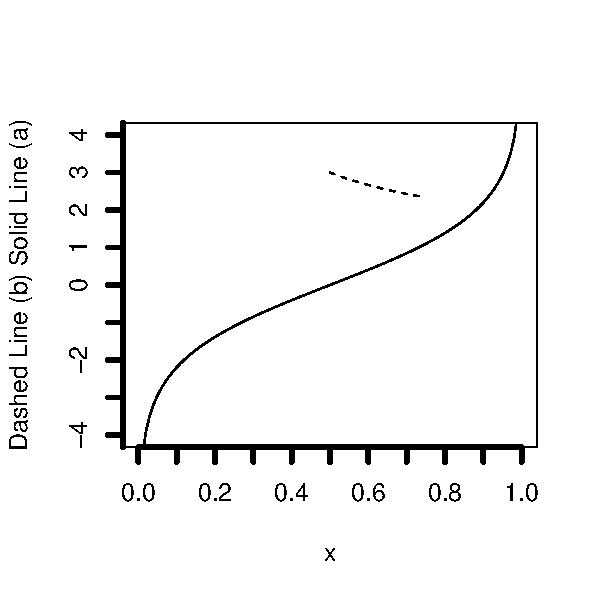
\includegraphics[width=\maxwidth]{figure/prob2xx-1} 

}



\end{knitrout}
\end{figure}


\end{enumerate}

\newpage

\item%3
Y $\sim$ POIS($\theta$)

$\theta$ $\sim$ GAM($\alpha$, $\beta$)

p($\theta \vert Y$) $\propto$ $\int_{\theta} \frac{\theta^{\Sigma y_{i}}\dot e^{-\theta}}{\Pi y_{i}!} \cdot \frac{\theta^{\alpha - 1}e^{-\frac{\theta}{\beta}}}{\Gamma(\alpha)\beta^{\alpha}} d\theta$

$\propto$ $\int_{\theta} \theta^{\Sigma y_{i} + \alpha - 1}\cdot e^{-\theta(1+\frac{1}{\beta})}$

$\theta \vert Y$ $\sim$ GAM($\Sigma y_{i} + \alpha$, $\frac{1}{1 +\frac{1}{\beta}}$)


\begin{enumerate}

\item%3a

Both posterior distributions are from the class of gamma distributions.

$\theta_{A} \vert Y \sim$ GAM(237,$\frac{1}{1.1}$)

$\theta_{B} \vert Y \sim$ GAM(125,$\frac{1}{2}$)


% latex table generated in R 3.3.1 by xtable 1.8-2 package
% Mon Sep 26 09:53:52 2016
\begin{table}[htb!]
\centering
\begin{tabular}{rrrrrrr}
  \hline
 & Posterior Shape & Posterior Scale & Posterior Mean & Posterior Variance & Lower Bound & Upper Bound \\ 
  \hline
A & 237.00 & 0.91 & 215.45 & 195.87 & 188.90 & 243.74 \\ 
  B & 125.00 & 0.50 & 62.50 & 31.25 & 52.02 & 73.92 \\ 
   \hline
\end{tabular}
\end{table}


\newpage

\item%3b


\begin{knitrout}
\definecolor{shadecolor}{rgb}{0.969, 0.969, 0.969}\color{fgcolor}
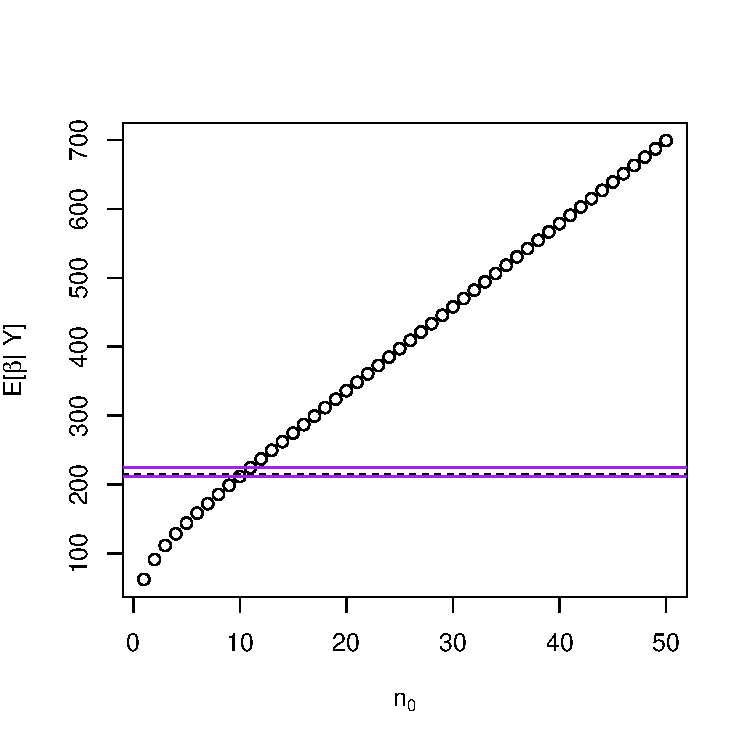
\includegraphics[width=\maxwidth]{figure/prob3b-1} 

\end{knitrout}

The solid lines represent the posterior expections of $\theta_{B}$ and the dashed line represents the posetior expectation of $\theta_{A}$ . The E[ $\theta_{A} \vert$ y] was 215.45. For the posterior of, $\theta_{B}$ to be be close to that of $\theta_{A}, n_{o}$ needs to be between 10 and 11, which lead to posterior expectations of  211.8182 and 224.5833 . Note that the priors on $\theta{A}$ and $\theta_{B}$ are the same if $n_{o}$ is 10, but different samples were observed for the two parameters, making the posterior expectations differ slightly.
\end{enumerate}


\item%4

Fisher's Information is $I(\theta)$. Binomial (which means Bernoulli as well) distributions are members of the exponential family, and so the regularity conditions hold. 

Where $\underset{\sim}{y} = \Sigma x_{i}$,

$I(\theta)$ = $-nE[(\frac{d^{2}}{d\theta^{2}}log(f(x\vert \theta)))]$

= $-E[(\frac{d^{2}}{d\theta^{2}}log(f(\underset{\sim}{y}\vert \theta)))]$

When $\underset{\sim}{y}\vert \theta \sim$ BIN(N,$\theta$)

$x\vert \theta \sim$ BERN($\theta$)

$I(\theta)$ = $-nE[(\frac{d^{2}}{d\theta^{2}}log(\theta^{x} \cdot (1 - \theta)^{1-x})]$

= $-nE[(\frac{d^{2}}{d\theta^{2}}[xlog(\theta) + (1-x)log(1 - \theta)]]$

= $-nE[(\frac{d}{d\theta})[\frac{x}{\theta} - (1 - \theta)^{-1} + \frac{x}{1 - \theta}]]$

= $-nE[\frac{-x}{\theta^{2}} - (1 - \theta)^{-2} + \frac{x}{(1 - \theta)^{2}}]$

= $-n[-\theta^{-1} - (1 - \theta)^{-2} + \frac{\theta}{(1 - \theta)^{2}}]$

= $-n[-\theta^{-1} - (1 - \theta)^{-1}]$

= $n[\theta^{-1} + (1 - \theta)^{-1}]$

= $n\frac{[(1 - \theta) + \theta]}{\theta(1-\theta)}$

= $\frac{n}{\theta(1-\theta)}$

Jeffrey's Prior $p_{j}(\theta)$ is then $(\frac{n}{\theta(1-\theta)})^{\frac{1}{2}}$

\end{enumerate}

\end{document}
